La primer etapa de experimentación consistió en verificar empíricamente la cota de complejidad temporal obtenida teóricamente para el algoritmo completo. Estas primeras cuatro figuras nos permiten ver que efectivamente nuestro algoritmo es $O(n * log(n))$

\begin{figure}[H]
    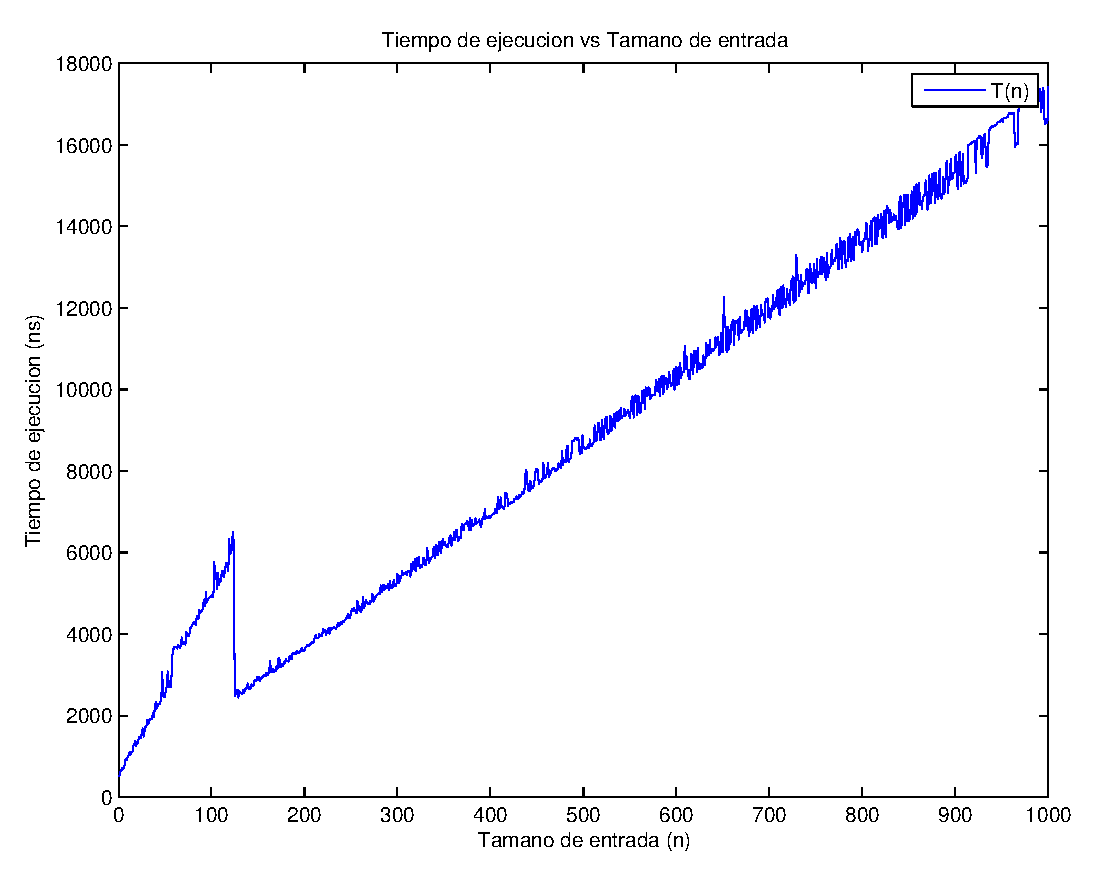
\includegraphics[width=0.5\linewidth]{problema1/graficos/problema1_aleatoria_1000.eps}
    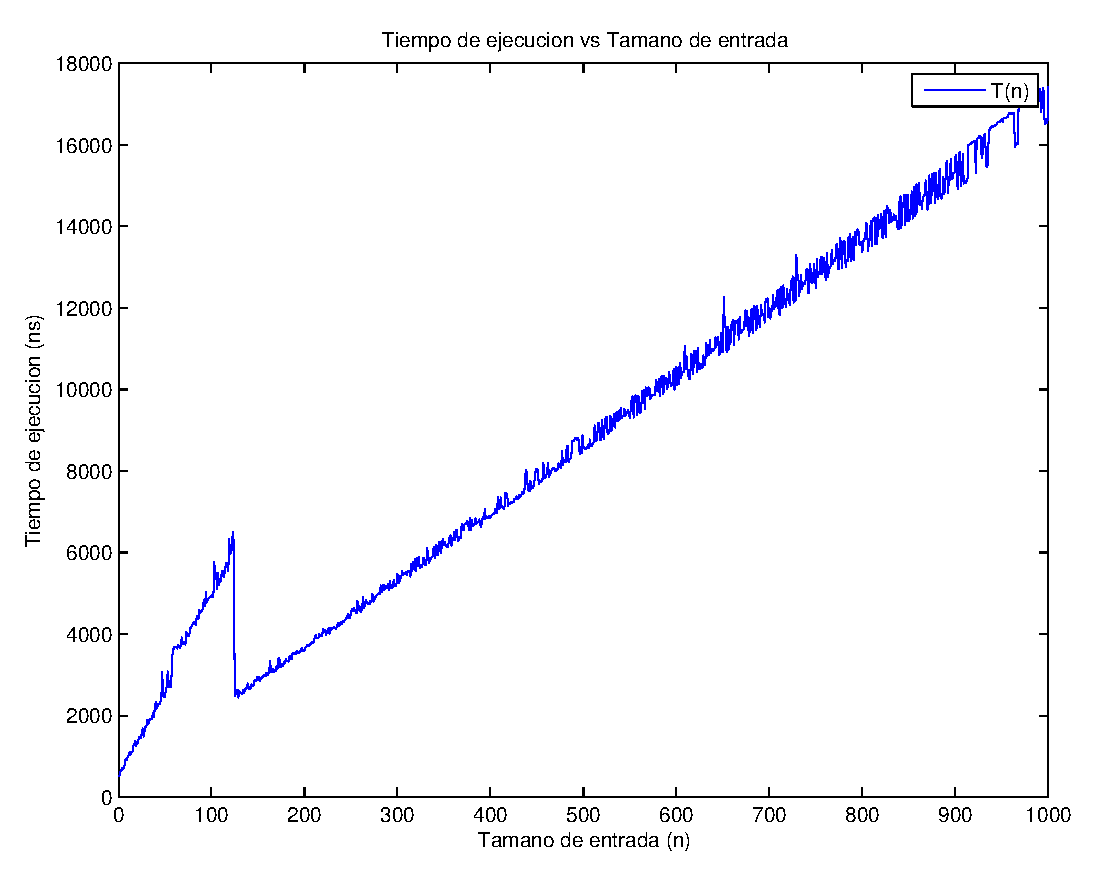
\includegraphics[width=0.5\linewidth]{problema1/graficos/problema1_aleatoria_1000.eps}
\end{figure}
\emph{\hspace{2,5cm}Figura 1: Caso n = 1000 \hspace{3cm}Figura 2: Idem, pero dividido por $log(n)$}

\begin{figure}[H]
    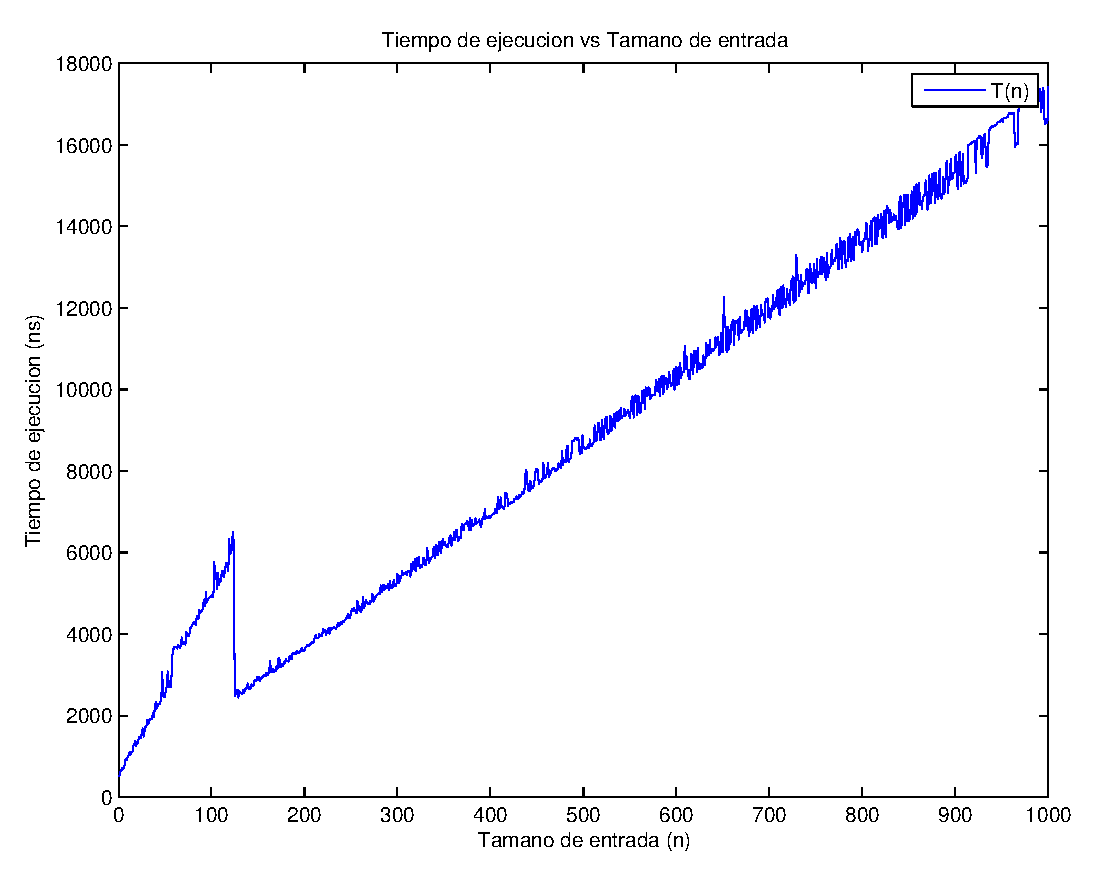
\includegraphics[width=0.5\linewidth]{problema1/graficos/problema1_aleatoria_1000.eps}
    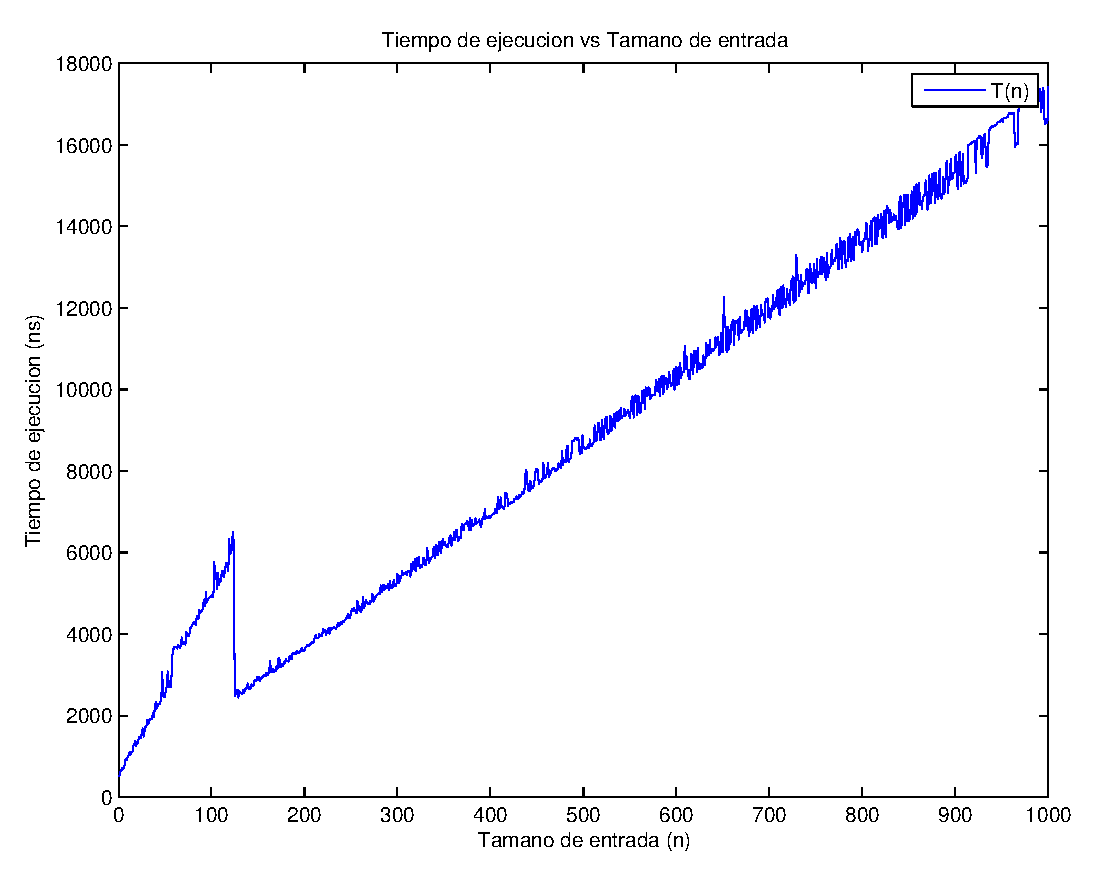
\includegraphics[width=0.5\linewidth]{problema1/graficos/problema1_aleatoria_1000.eps}
\end{figure}
\emph{\hspace{2,5cm}Figura 3: Caso n = 10000 \hspace{2,5cm}Figura 4: Idem, pero dividido por $log(n)$}

Como se puede observar en las figuras 2 y 4, una vez que dividimos por $log n$ nuestro algoritmo es una recta. Esto significa que la complejidad del algoritmo en su totalidad es de $O(n * log(n))$.

En los gráficos presentados arriba, se puede observar un pico alrededor de $n$ = 64. Como hablamos anteriormente, esto se debe al algoritmo de sorting que realiza un sorting especial con $n$ relativamente chico.

Según nuestro análisis, la complejidad temporal de la solución es dominada por la etapa de ordenamiento. Dado que el algoritmo utilizado para este fin pertenece a librerías estándares, la experimentación subsiguiente se realizó sobre instancias donde la lista de entrada se encuentra ordenada, eliminando la instrucción de ordenamiento. Esto permitió constatar si el ciclo final incurre efectivamente en un costo a lo sumo lineal, y verificar la preponderancia del ordenamiento como parte de la solución.

En las figuras siguientes podemos observar que, sin contar la etapa de ordenamiento, efectivamente nuestro algoritmo es $O(n)$. Para lograr esto, simplemente utilizamos entradas en las cuales los camiones estén ordenados, y por esto no haga falta realizar el sorting.

\begin{figure}[H]
    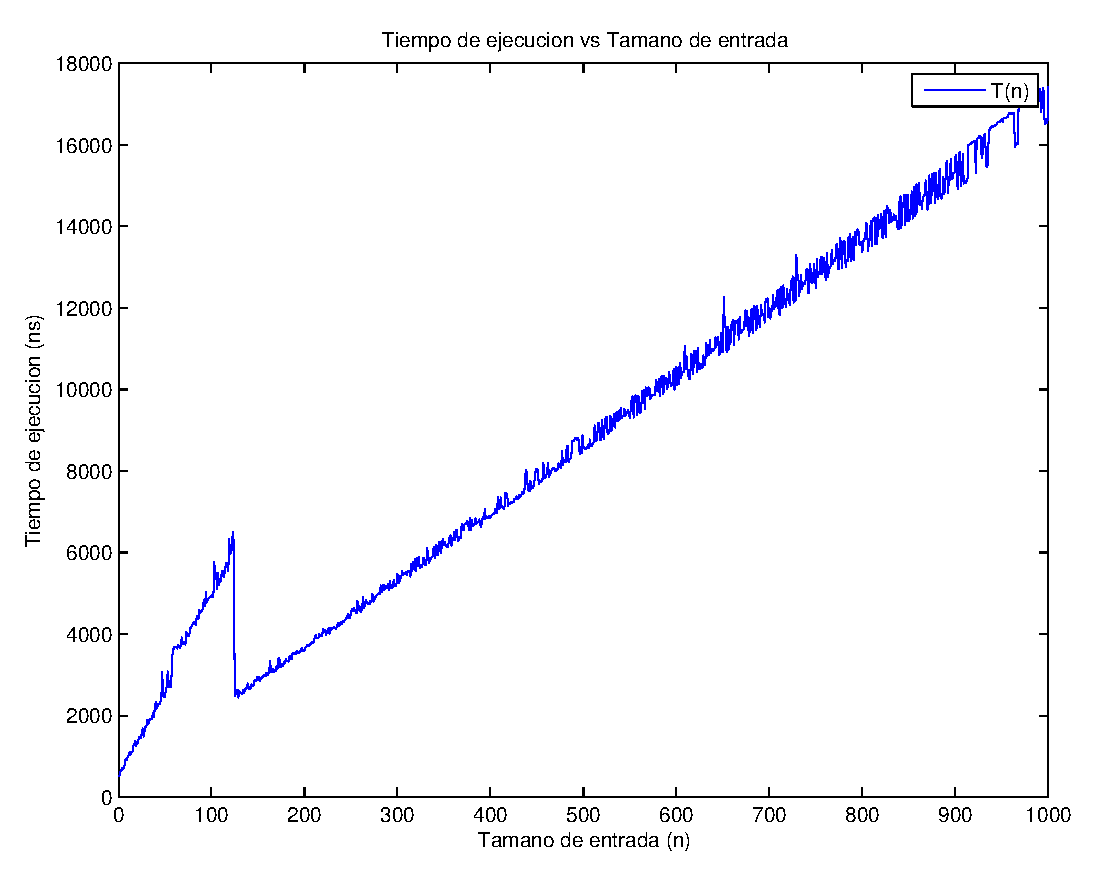
\includegraphics[width=0.5\linewidth]{problema1/graficos/problema1_aleatoria_1000.eps}
    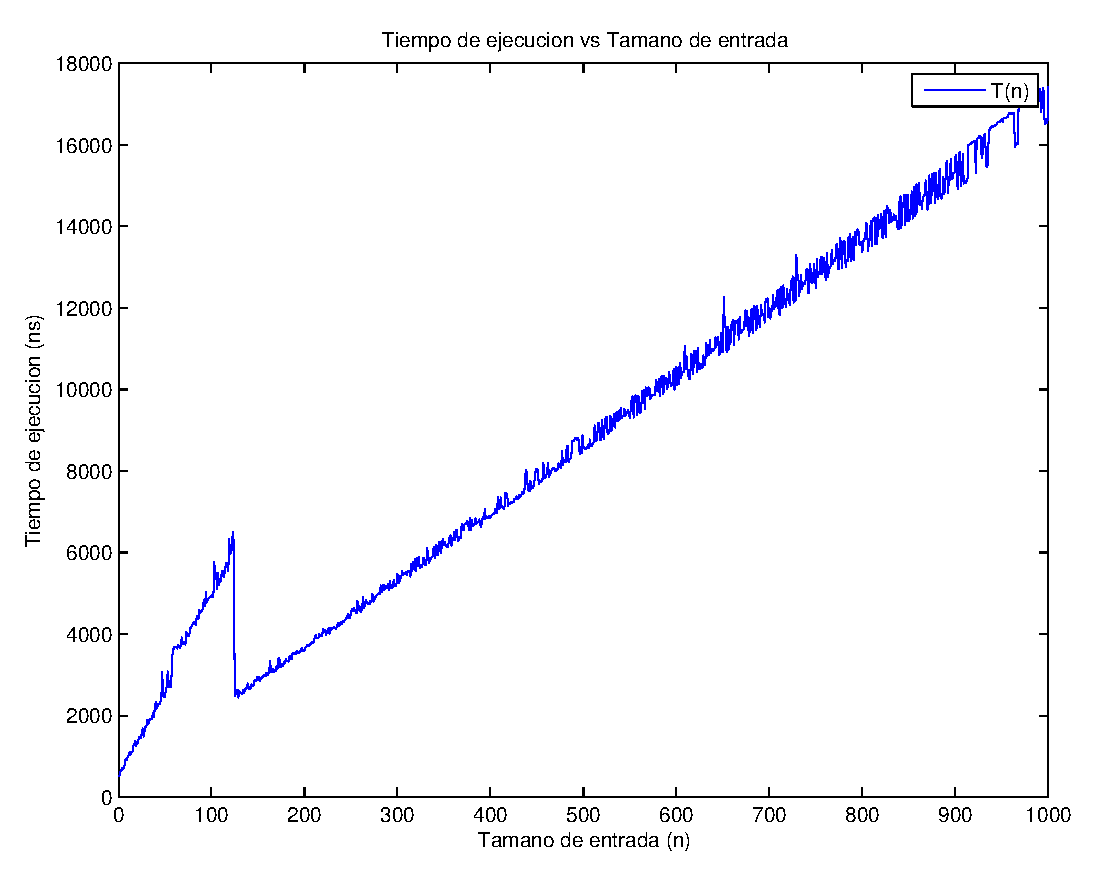
\includegraphics[width=0.5\linewidth]{problema1/graficos/problema1_aleatoria_1000.eps}
\end{figure}
\emph{\hspace{2cm}Figura 5: Caso n=1000, sin sorting \hspace{2,5cm}Figura 6: Idem, pero n=10000}
